\documentclass{beamer}
\usepackage{color}
\usepackage{booktabs}
\usepackage{multirow}
\usepackage{amssymb,graphicx}
\usepackage{pifont}

\begin{document}

\title{Multi-UAV Simulation Presentation}   
\author{Srijit Dutta\\} 
\date{\today} 


\frame{\titlepage} 
\section{Report} 



\subsection{Box2D}
\frame{\frametitle{Box-2D Simulation} 
\begin{itemize}
\item The scenario described in the paper, with a blimp and two copters is implemented
\item Fire is 'detected' in the simulation by sending a ball and monitoring its motion
\item Coordinated  motion is maintained between the copters monitoring the fire
\item Model involving a false alarm is also implemented in the simulation
\end{itemize}
}
%%%%%%%%%%%%%%%%%%%%%%%%%%%%%%%%%%%%%%%%%%%%%%%%          5%%%%%%%%%%%%
\subsection{Summary}
\frame{\frametitle{} 
\begin{itemize}
\item An overall coordinated movement is tried to be implemented
\end{itemize}

\begin{figure}[h!]
\centering
  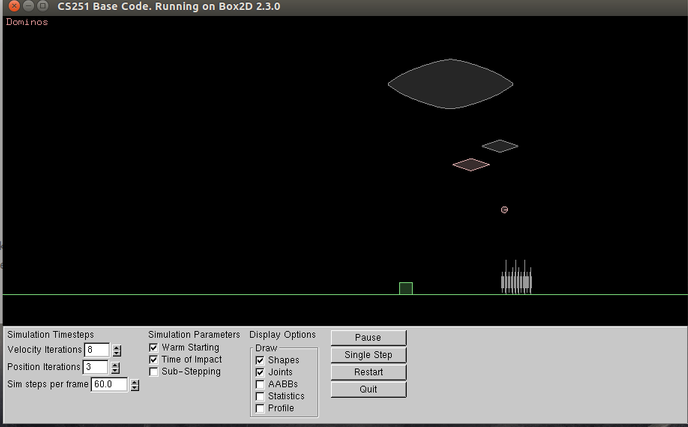
\includegraphics[width=80mm]{kgp2.png}
  \caption{Simulation}
  \label{fig:boat1}
\end{figure}
}
%%%%%%%%%%%%%%%%%%%%%%%%%%%
%%%%%%%%%%%%%%%%%%%%


\subsection{Cpp program}
\frame{\frametitle{Cpp Program} 
\begin{itemize}
\item The overall process of monitoring is shown here
\item The blimp performs detection over a area specified by the user
\item Two fires are determined randomly in the area specified
\item The true alarm is chosen by the user and the rest of the simulation works according to it
\end{itemize}
}

\subsection{Fire detect}
\frame{\frametitle{Fire Detection} 
\begin{itemize}
\item An executable for fire detection is provided which can detect presence of fire in photos and videos
\end{itemize}
\begin{figure}[h!]
\centering
  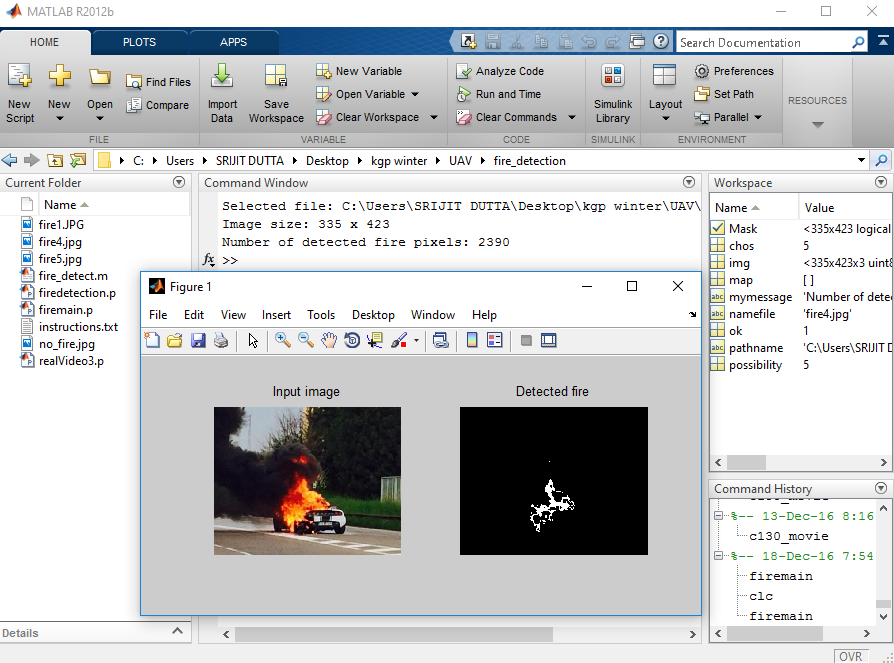
\includegraphics[width=80mm]{kgp1.png}
  \caption{Fire Detection}
  \label{fig:boat1}
\end{figure}
}
%%%%%%%%%%%%%%%%%%%%%%%%%%5
\subsection{Not Yet}
\frame{\frametitle{Yet to be Implemented} 
\begin{itemize}
\item Internal layers and structuring of UAVs have not been implemented in detail
\item  Integrating fire detection with Box2D simulation yet to be done
\item Machine level implementation not yet done
\end{itemize}
}
%%%%%%%%%%%%%%%%555


\end{document}